\documentclass[12pt]{article}

\usepackage[top=1in,bottom=1in,left=1in,right=1in]{geometry}
\usepackage{amsmath,amssymb,mathtools}
\usepackage{xcolor}
\usepackage{graphicx}
\usepackage{hyperref}
\usepackage{enumitem}

\hypersetup{
    pdfauthor={},
    pdftitle={MATH 1075 - Lesson 6.1 Recitation}
}

\begin{document}

\vspace*{0.5in}

\begin{center}
    {\LARGE MATH 1075 - Section 8.1 - 8.2 Worksheet}

    \vspace{2em}

    {\large 10/06/2026}
\end{center}
\section{Identifying Domain and Range}
Determine the domain and range.
\vspace{1.5em}

1. \begin{figure}[htbp]
    % Replace "my_image" with your actual file name (without extension)
    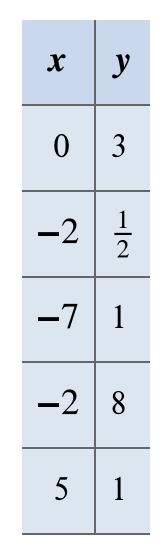
\includegraphics[width=0.12\linewidth]{Screenshot 2026-10-05 at 11.51.00 AM.png} 
\end{figure}

\vspace{3.5em}

2. \begin{figure}[htbp]
    % Replace "my_image" with your actual file name (without extension)
    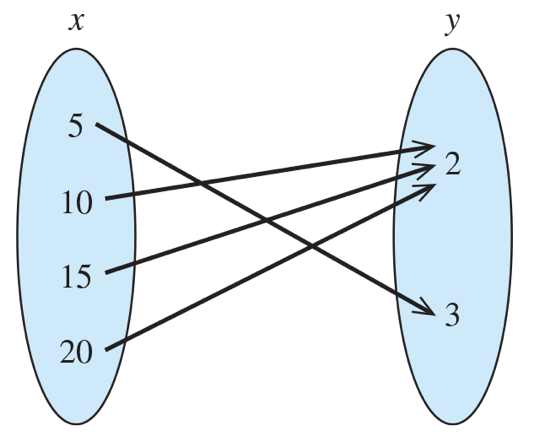
\includegraphics[width=0.4\linewidth]{Screenshot 2026-10-05 at 11.49.49 AM.png} 
\end{figure}

\newpage

3. \begin{figure}[htbp]
    % Replace "my_image" with your actual file name (without extension)
    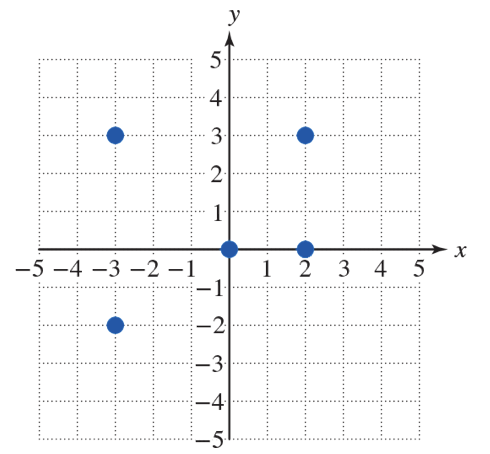
\includegraphics[width=0.5\linewidth]{Screenshot 2026-10-05 at 11.54.07 AM.png} 
\end{figure}

\vspace{3.5em}

4. \begin{figure}[htbp]
    % Replace "my_image" with your actual file name (without extension)
    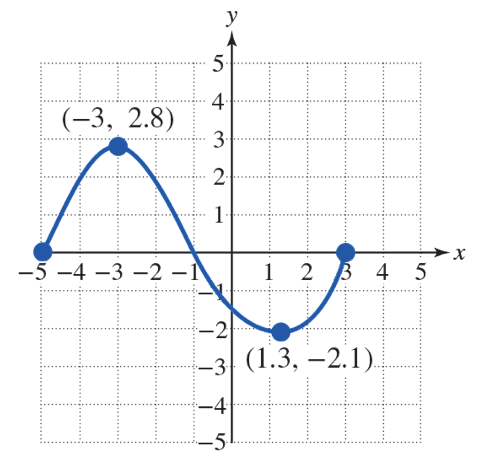
\includegraphics[width=0.5\linewidth]{Screenshot 2026-10-05 at 11.55.59 AM.png} 
\end{figure}

\newpage 

5. \begin{figure}[htbp]
    % Replace "my_image" with your actual file name (without extension)
    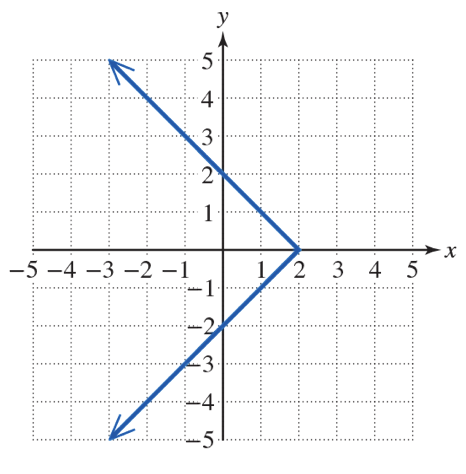
\includegraphics[width=0.5\linewidth]{Screenshot 2026-10-05 at 11.57.27 AM.png} 
\end{figure}

\vspace{3.5em}
6. \begin{figure}[htbp]
    % Replace "my_image" with your actual file name (without extension)
    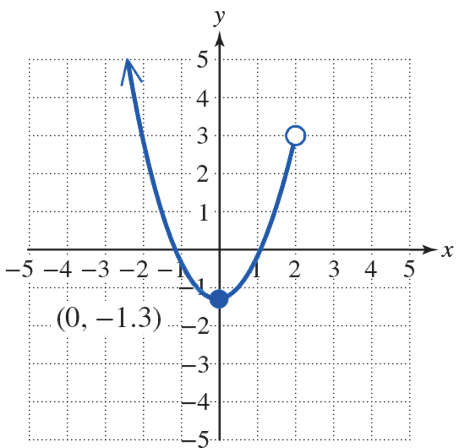
\includegraphics[width=0.52\linewidth]{Screenshot 2026-10-05 at 11.58.51 AM.png} 
\end{figure}

\newpage

\section{Function}
Determine if the relation defines $y$ as a function of $x.$
\vspace{1.5em}

1. $\{(1,2),(2,3),(3,4),(4,5)\}$

\vspace{3.5em}
2. $\{(1,4),(2,5),(4,6),(5,7),(4,10)\}$

\vspace{3.5em}

3.\begin{figure}[htbp]
    % Replace "my_image" with your actual file name (without extension)
    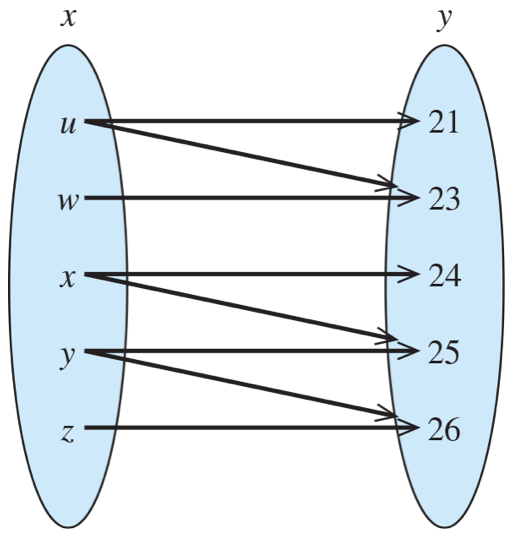
\includegraphics[width=0.4\linewidth]{Screenshot 2026-10-05 at 12.24.43 PM.png} 
\end{figure}

\vspace{3.5em}

4. \begin{figure}[htbp]
    % Replace "my_image" with your actual file name (without extension)
    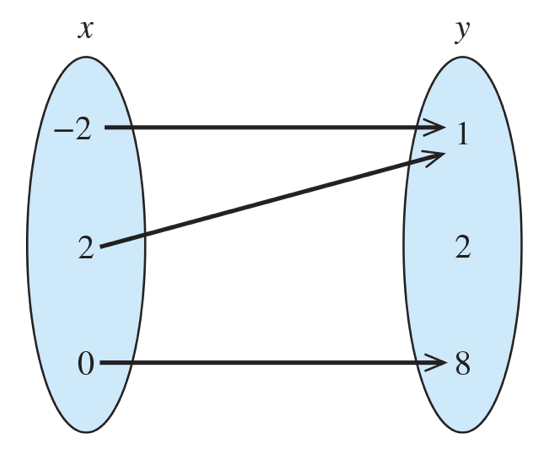
\includegraphics[width=0.4\linewidth]{Screenshot 2026-10-05 at 12.27.26 PM.png} 
\end{figure}
\newpage 
5. \begin{figure}[htbp]
    % Replace "my_image" with your actual file name (without extension)
    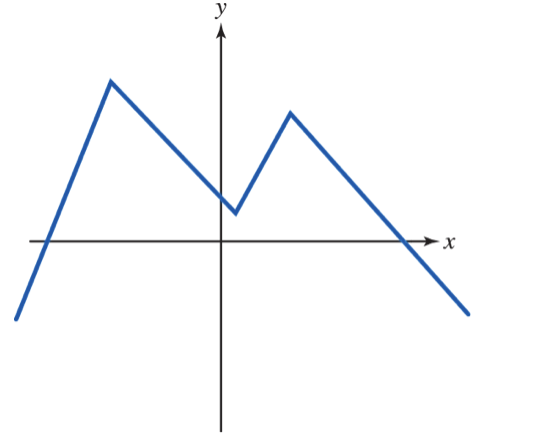
\includegraphics[width=0.5\linewidth]{Screenshot 2026-10-05 at 12.29.19 PM.png} 
\end{figure}

\vspace{3.5em}

6. \begin{figure}[htbp]
    % Replace "my_image" with your actual file name (without extension)
    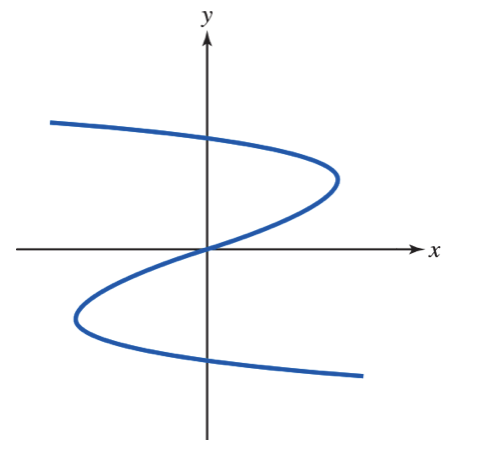
\includegraphics[width=0.5\linewidth]{Screenshot 2026-10-05 at 12.30.22 PM.png} 
\end{figure}
\newpage 
\section{Function Notation and Evaluating Function}
Given a function $f(x)=x^{2}+2x+1$ find: 
\vspace{1.5em}

1. $f(1)$

\vspace{3.5em}

2. $f(-1)$

\vspace{3.5em}

3. $f(0)$

\vspace{3.5em}

4. $f(5)$

\vspace{3.5em}

\noindent Given a graph of a function $K(x),$ find:

\begin{figure}[htbp]
    % Replace "my_image" with your actual file name (without extension)
    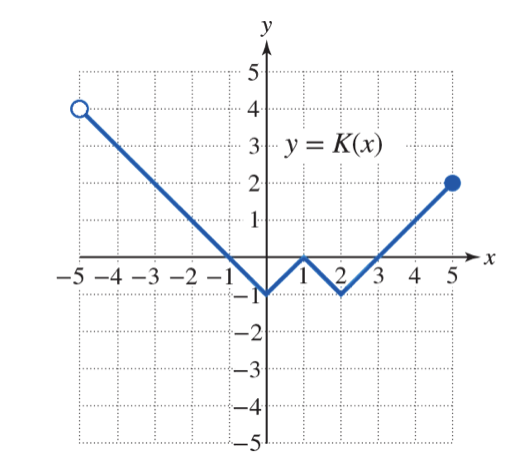
\includegraphics[width=0.5\linewidth]{Screenshot 2026-10-05 at 12.50.41 PM.png} 
\end{figure}
5. $K(1)$ 

\vspace{3.5em}

6. $K(0)$ 

\vspace{3.5em}

7. $K(5)$

\newpage 
\section{Domain of Function} 
Find domain of each function. 
\vspace{1.5em}

1. $f(x)=\frac{(x+1)^{2}}{(x+1)} $ 

\vspace{3.5em}

2. $g(x)=\frac{5x-1}{x^{2}+1} $ 

\vspace{3.5em}

3. $h(x)=\sqrt{x+5}$ 

\vspace{3.5em}

4. $k(x)=\frac{1}{\sqrt{x+5}} $ 

\end{document}
